\documentclass{beamer}
\usepackage{etex}
\reserveinserts{28}

\usepackage{fancyvrb}
\usepackage{color, colortbl}
\usepackage{listings}
\usepackage{url}
\usepackage{array}
\usepackage{calc}
\usepackage{ctable}
\usepackage{amsmath}
\usepackage{cite}
\usepackage{graphicx}
\usepackage{listings}
\usepackage{xspace}
\usepackage{hyperref}
\usepackage{subfigure}
\usepackage{multicol}
\definecolor{lightgray}{rgb}{0.9,0.9,0.9}



\lstset{ %
language=C++,                % choose the language of the code
basicstyle=\tiny,       % the size of the fonts that are used for the code
%numbers=left,                   % where to put the line-numbers
numbers=none,                   % where to put the line-numbers
numberstyle=\scriptsize,      % the size of the fonts that are used for the line-numbers
stepnumber=1,                   % the step between two line-numbers. If it's 1 each line will be numbered
numbersep=15pt,                  % how far the line-numbers are from the code
backgroundcolor=\color{lightgray},  % choose the background color. You must add \usepackage{color}
%backgroundcolor=none,  % choose the background color. You must add \usepackage{color}
showspaces=false,               % show spaces adding particular underscores
showstringspaces=false,         % underline spaces within strings
showtabs=false,                 % show tabs within strings adding particular underscores
frame=single,	                % adds a frame around the code
%frame=none,	                % adds a frame around the code
tabsize=2,	                % sets default tabsize to 2 spaces
%captionpos=b,                   % sets the caption-position to bottom
captionpos=n,
%basicstyle=\small,
%basicstyle=\small\sffamily,
basicstyle=\sffamily\small,
%basicstyle=\ttfamily\small,
breaklines=true,                % sets automatic line breaking
breakatwhitespace=false,        % sets if automatic breaks should only happen at whitespace
columns=fullflexible,
title=\lstname,                 % show the filename of files included with \lstinputlisting; also try caption instead of title
escapeinside={\%*}{*)},          % if you want to add a comment within your code
morekeywords={chare,mainchare,module,mainmodule,entry,readonly,array,serial,for,when,if,then,else,overlap,while,forall,threaded,sync,message,group,nodegroup},
aboveskip=2pt,
belowskip=2pt,
lineskip=0pt,
xleftmargin=1em,
xrightmargin=1em,
%xleftmargin=10pt
abovecaptionskip=0pt,
belowcaptionskip=0pt,
}

\hypersetup{
    colorlinks,%
    citecolor=black,%
    filecolor=black,%
    linkcolor=black,%
    urlcolor=magenta
}


\usefonttheme{professionalfonts}
\usetheme{Boadilla}
\usecolortheme{beaver}

%\AtBeginSubsection[]
%{
%    \begin{frame}{Outline}
%        \tableofcontents[currentsection,currentsubsection]
%    \end{frame}
%}

\AtBeginSection[]{
%  \setbeamercolor{section in toc shaded}{use=structure,fg=structure.fg}
%  \setbeamercolor{section in toc}{fg=mycolor}
%  \setbeamercolor{subsection in toc shaded}{fg=black}
%  \setbeamercolor{subsection in toc}{fg=mycolor}
  \frame<beamer>{\begin{multicols}{2}
  \frametitle{Outline}
  \setcounter{tocdepth}{2}  
%  \tableofcontents[currentsection,subsections]
  \tableofcontents[currentsection,currentsubsection]
\end{multicols} 
 }
}


\newcommand{\charm}{Charm++}
\newcommand{\code}[1]{\colorbox{lightgray}{\texttt{#1}}}
\newcommand{\transition}[1]{\begin{frame}[plain]\begin{center}\LARGE #1\end{center}\end{frame}}
\newcommand{\comment}[1]{ }
\newcommand{\eat}[1]{ }

\DefineVerbatimEnvironment{codeverb}{Verbatim}{fontsize=\small}

\let \isForClass 1
\if \isForClass 1
  \newcommand{\removeForClass}[2]{#2}
  \else
  \newcommand{\removeForClass}[2]{#1}
\fi


\title{Basic Charm++}

\author[Laxmikant V.~Kale]{
Laxmikant V.~Kale
}
\date{\today}

\begin{document}

\begin{frame}[fragile]
  \frametitle{Chare Arrays}
  \begin{itemize}
    \item Indexed collections of chares
      \begin{itemize}
      \item Every item in the collection has a unique index and proxy
      \item Can be indexed like an array or by an arbitrary object
      \item Can be sparse or dense
      \item Elements may be dynamically inserted and deleted
      \end{itemize}
    \item For many scientific applications, collections of chares are a
      convenient abstraction
    \item Instead of creating networks of chares that learn about each other
      (by sending proxies to each other), each element in a chare array knows
      about all the others
  \end{itemize}
\end{frame}

\begin{frame}
  \frametitle{Chare Array Location}
  \begin{itemize}
  \item By default, chare arrays are distributed to the processors in a
    ``blocked'' distribution
  \end{itemize}
  \begin{center} 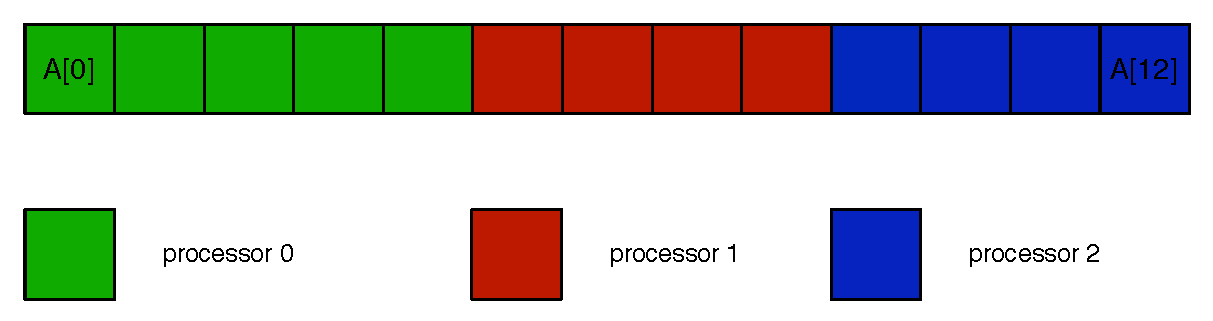
\includegraphics[width=0.8\textwidth]{figures/blockedDist.pdf} \end{center}
  \begin{itemize}
  \item A initial mapping function can be specified (input is the index, output
    is the processor)
    \begin{itemize}
    \item Called the \emph{home PE} of the element
    \end{itemize}
  \item Chare array elements can be migrated by the user or the runtime (load balancing)
  \end{itemize}
\end{frame}



\begin{frame}[fragile]
  \frametitle{Declaring a Chare Array}
  \texttt{.ci} file:
  \begin{lstlisting}
    array [1d] foo {
      entry foo(); // constructor
      // ... entry methods ...
    }
    array [2d] bar {
      entry bar();  // constructor
      // ... entry methods ...
    }
  \end{lstlisting}
  \texttt{.C} file:

  \begin{lstlisting}
    struct foo : public CBase_foo {
      foo() { }
      foo(CkMigrateMessage*) { }
    };
    struct bar : public CBase_bar {
      bar() { }
      bar(CkMigrateMessage*) { }
    };
  \end{lstlisting}
\end{frame}

\begin{frame}[fragile]
  \frametitle{Constructing a Chare Array}
  \begin{itemize}
    \item Constructed much like a regular chare
    \item The size of each dimension is passed to the constructor
  \end{itemize}
  \begin{lstlisting}
    void someMethod() {
       CProxy_foo::ckNew(10);
       CProxy_bar::ckNew(5, 5);
    }
  \end{lstlisting}
  \begin{itemize}
  \item The proxy may be retained:
  \end{itemize}
  \begin{lstlisting}
    CProxy_foo myFoo = CProxy_foo::ckNew(10);
  \end{lstlisting}
  \begin{itemize}
  \item The proxy represents the entire array, and may be indexed to obtain a
    proxy to an individual element in the array
  \end{itemize}
  \begin{lstlisting}
    CProxyElement_foo elm = myFoo[5];
    elm.invokeEntry();
    myFoo[4].invokeEntry();
  \end{lstlisting}
\end{frame}

\begin{frame}[fragile]
  \frametitle{\code{thisIndex}}
  \begin{itemize}
  \item 1d: \code{thisIndex} returns the index of the current chare array element
  \item 2d: \code{thisIndex.x} and \code{thisIndex.y} returns the indices of
    the current chare array element
  \end{itemize}
  \texttt{.ci} file:
  \begin{lstlisting}
    array [1d] foo {
      entry foo();
    }
  \end{lstlisting}

  \texttt{.C} file:
  \begin{lstlisting}
    struct foo : public CBase_foo {
      foo() {
        CkPrintf("array index = %d", thisIndex);
      }
    };
  \end{lstlisting}

\end{frame}

\removeForTutorial{
\begin{frame}[fragile]
  \frametitle{Chare Array: Hello Example }
  \lstinputlisting{code/arrayHello.ci}
\end{frame}

\begin{frame}[fragile]
  \frametitle{Chare Array: Hello Example }
  \lstinputlisting[basicstyle=\scriptsize]{code/arrayHello.cpp}
\end{frame}

\begin{frame}[fragile]
   \frametitle{Hello World Array Projections Timeline View}\scriptsize
  \begin{itemize}
    \item Add \texttt{-tracemode projections} to link line to enable tracing
    \item Run Projections tool to load trace log files and visualize performance
  \end{itemize}
  \begin{center} 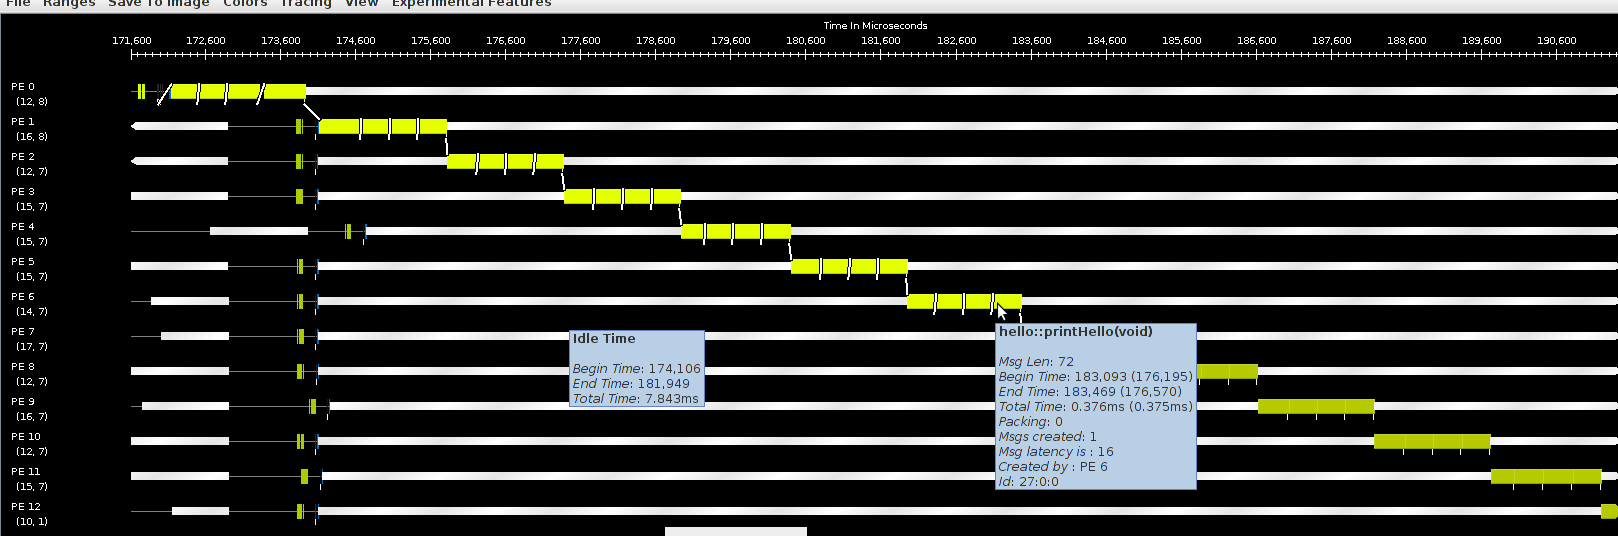
\includegraphics[width=0.99\textwidth]{figures/arrayHelloTimeline} \end{center}
  \begin{itemize}
   \item arrayHello on BG/Q 16 Nodes, mode c16, 1024 elements (4 per process)
  \end{itemize}
\end{frame}



}

\begin{frame}[fragile]
  \frametitle{Collections of Objects: Runtime Service}
  \begin{itemize}
    \item System knows how to `find' objects efficiently: $(collection, index) \to processor$
    \item Applications can specify a mapping, or use simple
      runtime-provided options (e.g. blocked, round-robin)
    \item Distribution can be static, or dynamic!
    \item Key abstraction: application logic doesn't change, even
      though performance might
  \end{itemize}
\end{frame}

\begin{frame}[fragile]
  \frametitle{Collections of Objects: Runtime Service}
  \begin{itemize}
    \item Can develop and test logic in objects separately from their distribution
    \item Separation in time: make it work, then make it fast
    \item Division of labor: domain specialist writes object code, computationalist writes mapping
    \item Portability: different mappings for different systems, scales, or configurations
    \item Shared progress: improved mapping techniques can benefit existing code
  \end{itemize}
\end{frame}

\begin{frame}[fragile]
  \frametitle{Collections of Objects}
  \begin{center}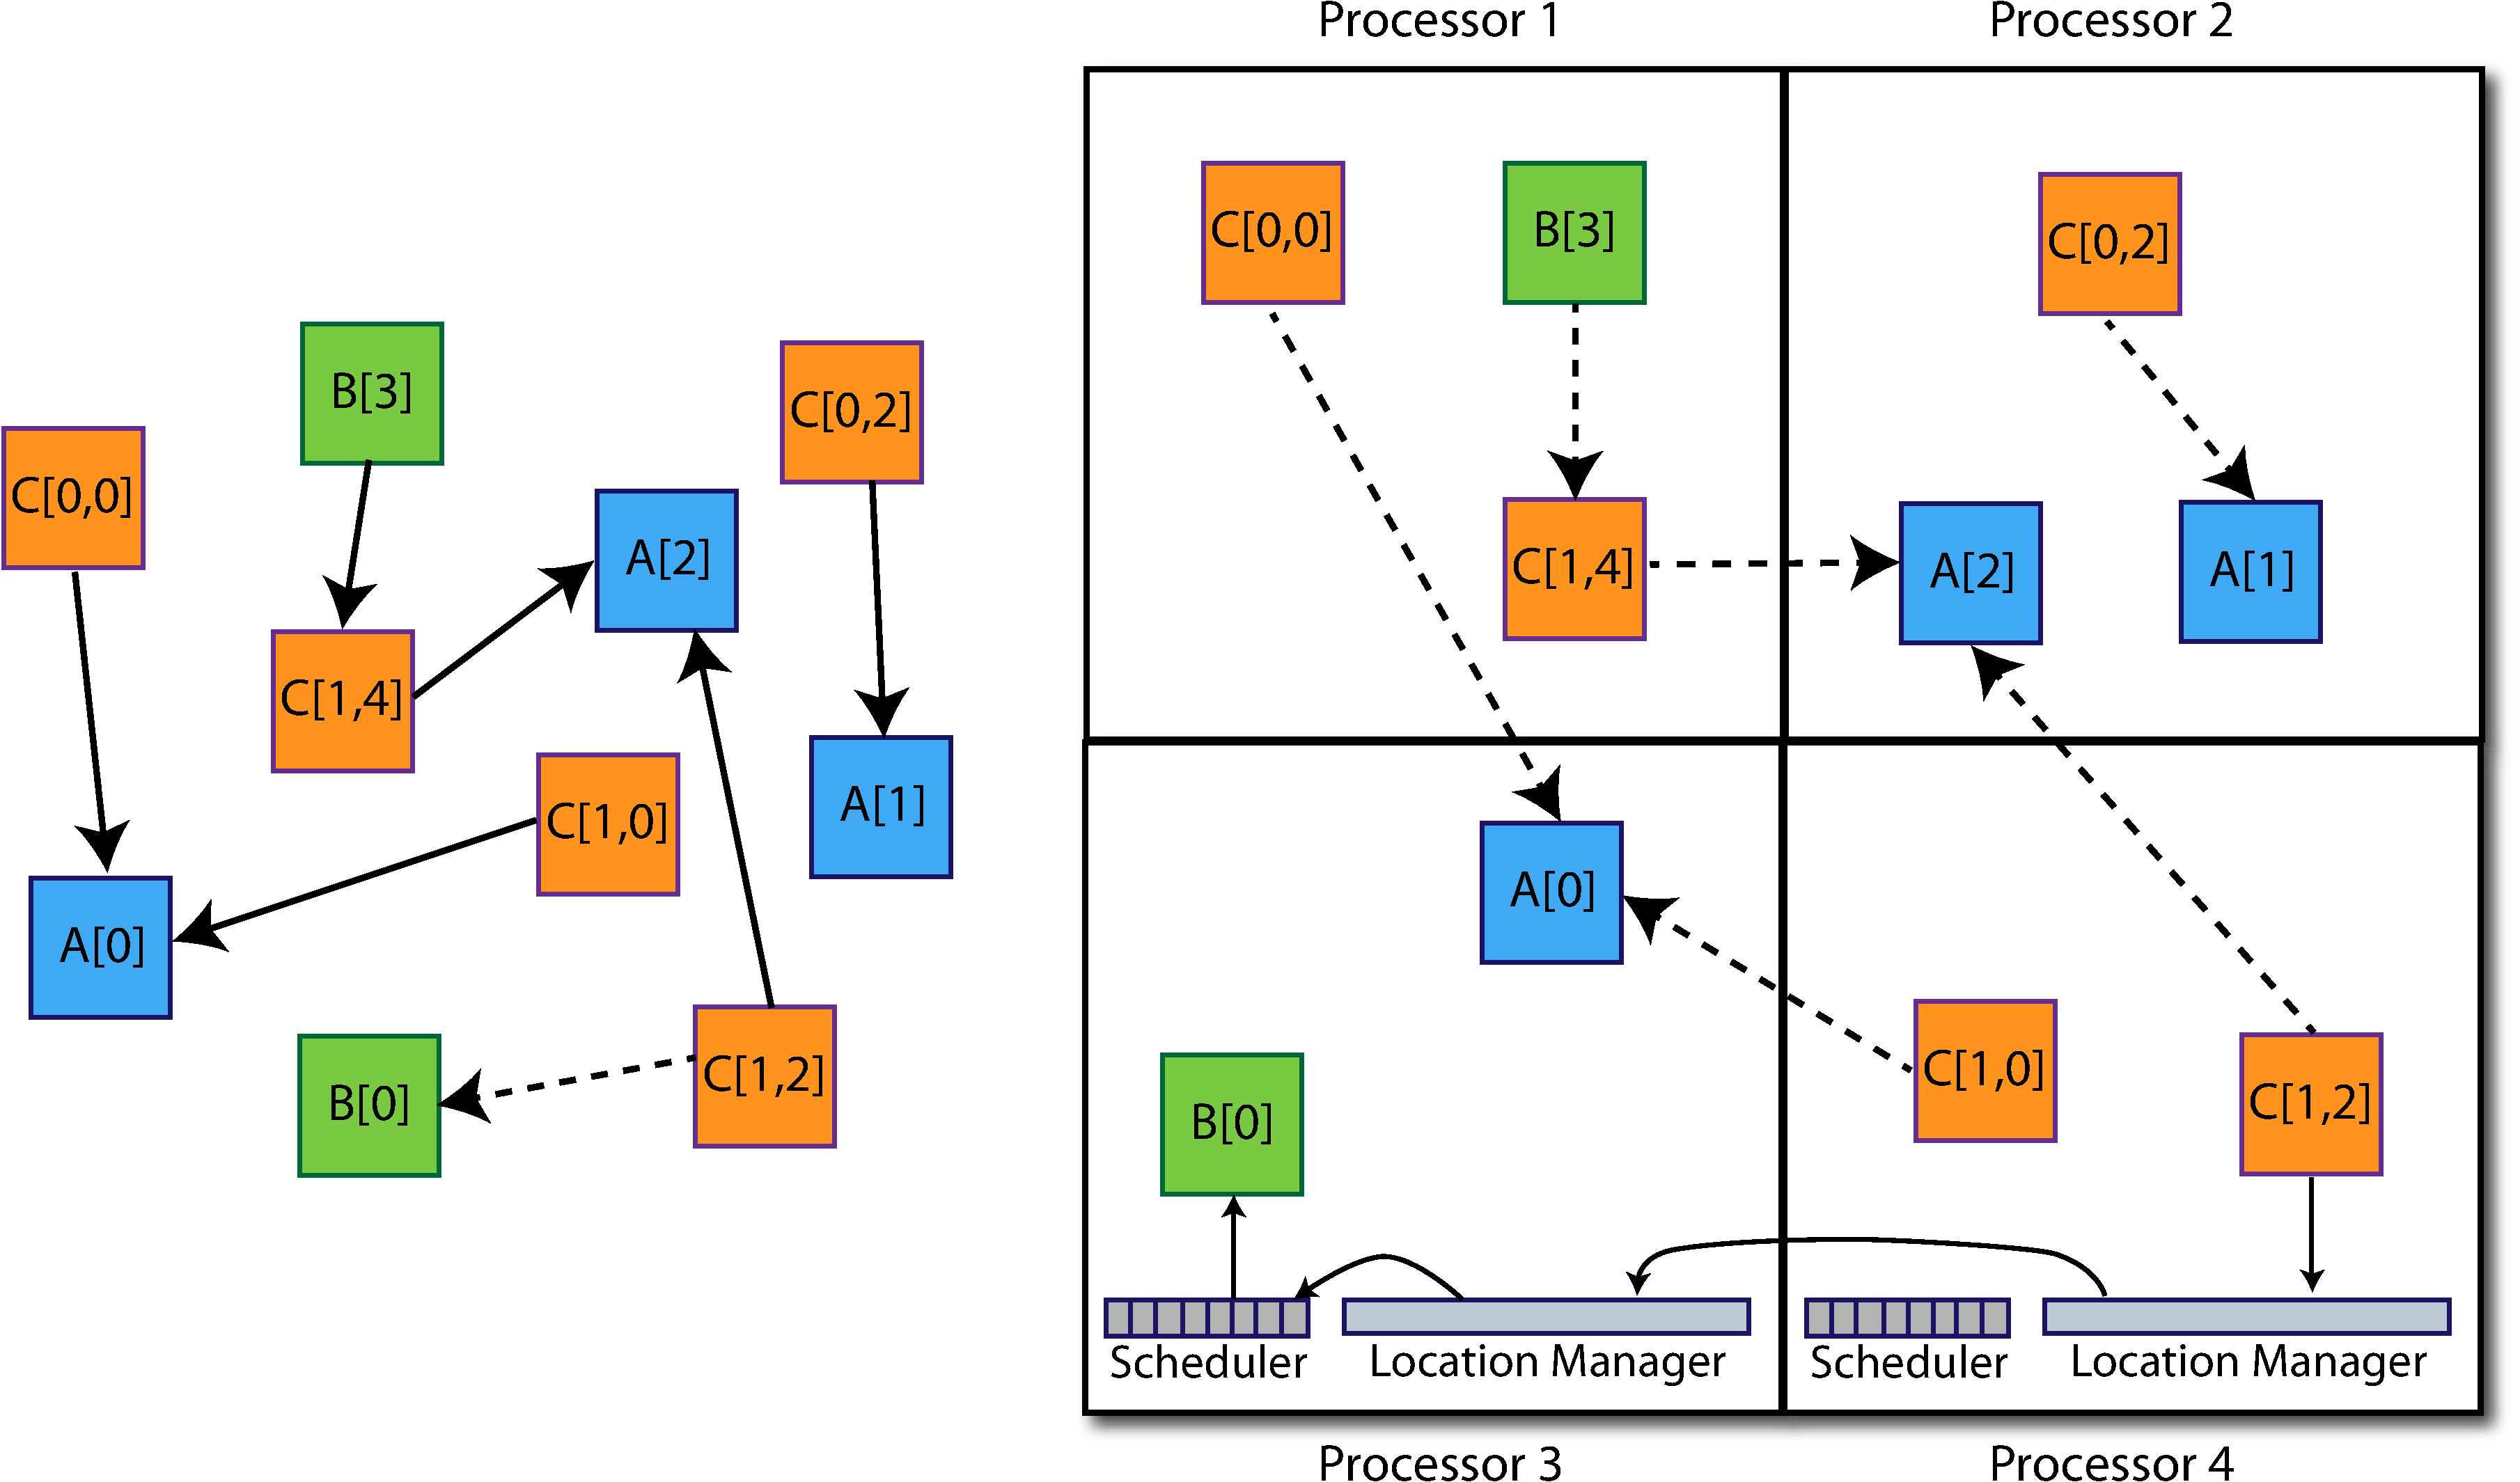
\includegraphics[width=0.9\textwidth]{figures/elements2.pdf}\end{center}
\end{frame}

\begin{frame}[fragile]
  \frametitle{Collective Communication Operations}
  \begin{itemize}
    \item Point-to-point operations involve only two objects
    \item Collective operations that involve a collection of objects
    \item Broadcast: calls a method in each object of the array
    \item Reduction: collects a contribution from each object of the array
    \item A spanning tree is used to send/receive data
  \end{itemize}
    \begin{center} 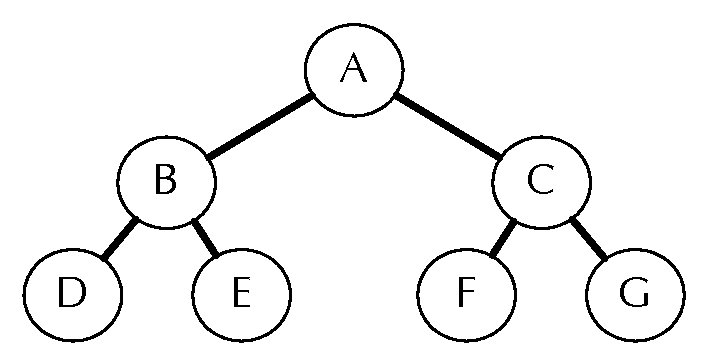
\includegraphics[width=0.5\textwidth]{figures/spanningTree.pdf} \end{center}
\end{frame}


\begin{frame}[fragile]
  \frametitle{Broadcast}
  \begin{itemize}
    \item A message to each object in a collection
    \item The chare array proxy object is used to perform a broadcast
    \item It looks like a function call to the proxy object
    \item From the main chare:
    \begin{lstlisting}
CProxy_Hello helloArray = CProxy_Hello::ckNew(helloArraySize);
helloArray.foo();
    \end{lstlisting}
    \item From a chare array element that is a member of the same array:
     \begin{lstlisting}
 thisProxy.foo()
    \end{lstlisting}
  \end{itemize}
\end{frame}

\begin{frame}[fragile]
  \frametitle{Reduction}
  \begin{itemize}
  \item Combines a set of values: sum, max, aggregate
  \item Usually reduces the set of values to a single value
  \item Combination of values requires an operator
  \item The operator must be commutative and associative
  \item Each object calls \code{contribute} in a reduction
  \end{itemize}
\end{frame}

\begin{frame}[fragile]
  \frametitle{Reduction: Example}
  \lstinputlisting{code/reductionMainTarget.ci}
\end{frame}

\begin{frame}[fragile]
  \frametitle{Reduction: Example}
  \lstinputlisting[basicstyle=\tiny]{code/reductionMainTarget.cpp}
Output:
  \begin{lstlisting}[basicstyle=\tiny]
value: 1176
Program finished.
  \end{lstlisting}
\end{frame}

\removeForClass{
\begin{frame}[fragile]
  \frametitle{Quick Hands-on}
  \begin{itemize}
  \item Log onto your vesta account.
  \item Obtain the following code:\\ git clone git://charm.cs.uiuc.edu/users/tutorial\_exercise
  \item Read the README.
  \item Change to toy directory, and read assignment.txt.
  \item Uncomment the CHARMC declaration at top of Makefile and make.
  \item ./charmrun -A $<$your\_account$>$ +p4 ./hello 16.
  \item Modify paramter to be an array instead of int.
  \end{itemize}
\end{frame}
}

%comment for removeForClass macro to work


\begin{frame}[fragile]
  \frametitle{Parallel Prefix Example: main.ci}
  \lstinputlisting{code/par-prefix-no-sdag/main.ci}
\end{frame}

\begin{frame}[fragile]
  \frametitle{Parallel Prefix Example: main.h}
  \lstinputlisting[basicstyle=\tiny]{code/par-prefix-no-sdag/main.h}
\end{frame}

\begin{frame}[allowframebreaks]
  \frametitle{Parallel Prefix Example: main.C}
  \lstinputlisting[basicstyle=\tiny]{code/par-prefix-no-sdag/main.C}
\end{frame}

\begin{frame}[fragile]
  \frametitle{Parallel Prefix Example: prefix.ci}
  \lstinputlisting{code/par-prefix-no-sdag/prefix.ci}
\end{frame}

\begin{frame}[allowframebreaks]
  \frametitle{Parallel Prefix Example: prefix.h}
  \lstinputlisting[basicstyle=\tiny]{code/par-prefix-no-sdag/prefix.h}
\end{frame}

\begin{frame}[allowframebreaks]
  \frametitle{Parallel Prefix Example: prefix.C}
  \lstinputlisting[basicstyle=\tiny]{code/par-prefix-no-sdag/prefix.C}
\end{frame}

\end{document}
